\documentclass[12pt]{ctexart}

\title{Parallel Homework \#3}
\author{刘康来}
%\data{\today}

\usepackage{graphicx}
\graphicspath{{./}}
%\usepackage{listings}


\begin{document}

\maketitle

\newpage

\begin{figure}[h!]
    \centering
    \caption{Here is the hardware's information}
    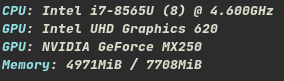
\includegraphics[scale=0.5]{HardwareInfo}
    \caption{About the GPU and CUDA}
    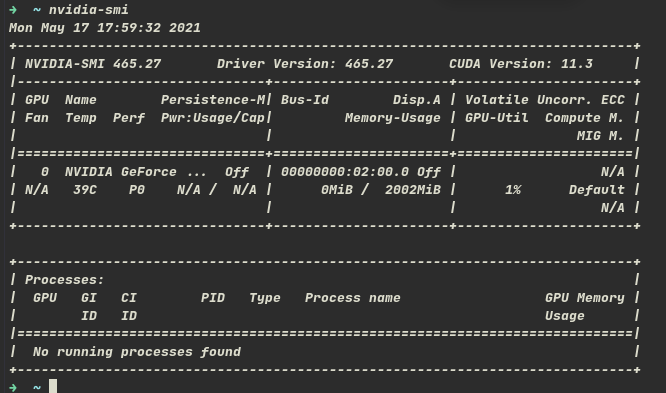
\includegraphics[scale=0.5]{Gpu}
    \caption{Here is the test runnig}
    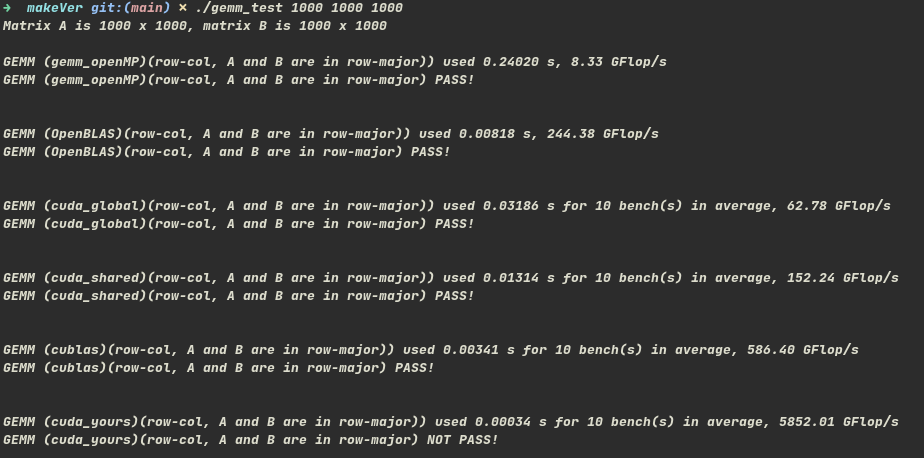
\includegraphics[scale=0.5]{testrunning}
\end{figure}

\newpage

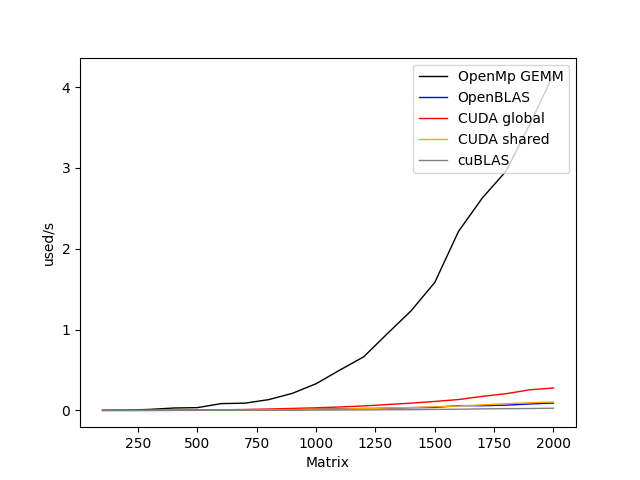
\includegraphics[scale=0.5]{1s}
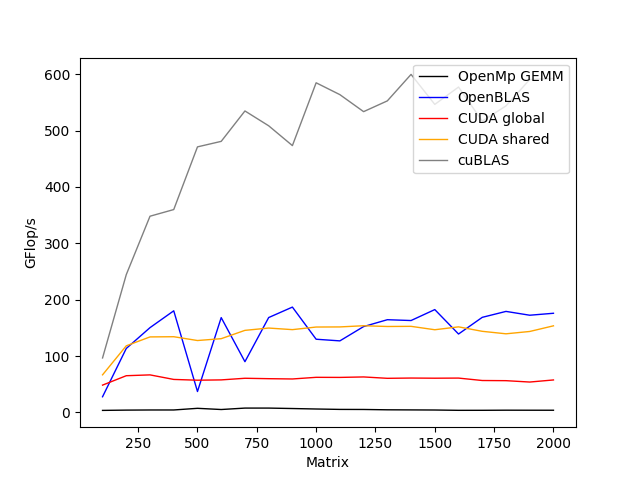
\includegraphics[scale=0.5]{1g}

As you can see, the cuBLAS is the fastest, than is OpenBLAS, CUDA using shared memory, CUDA using global memory and basic code using OpenMP.

For better comparison, I use the given remote device to run the code(the Matrix from 2100 to 3500).\\Here is the result:

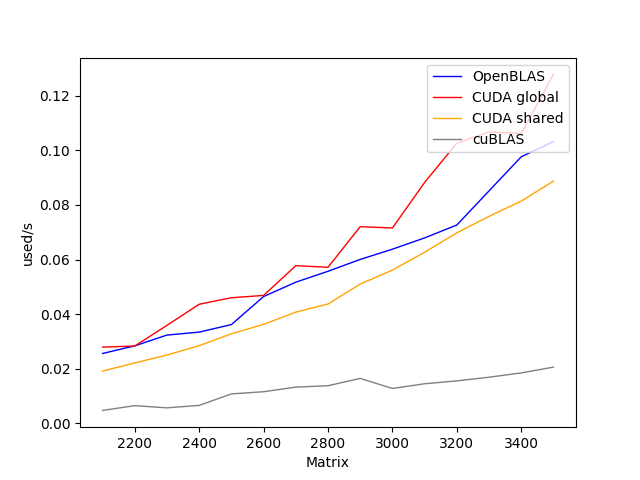
\includegraphics[scale=0.5]{2s}
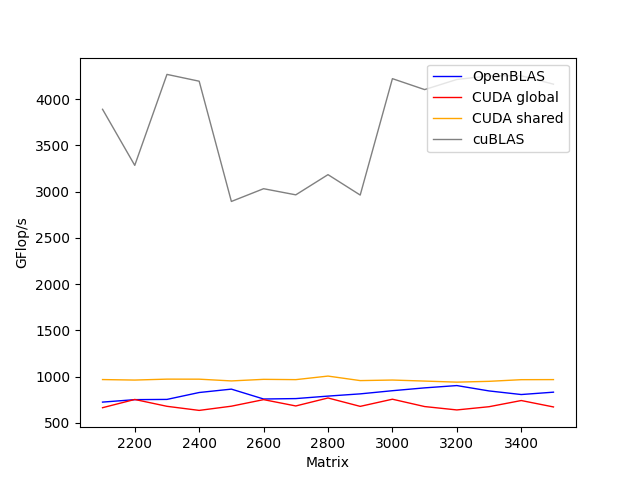
\includegraphics[scale=0.5]{2g}

\newpage

The CUDA GEMM code optimized by yourself with your own techniques...
\\In theory, using more blocks is better, but cost more memory. I try the BLOCK\_SIZE 4, 8, 16, 32 to run the code, here is the performance:

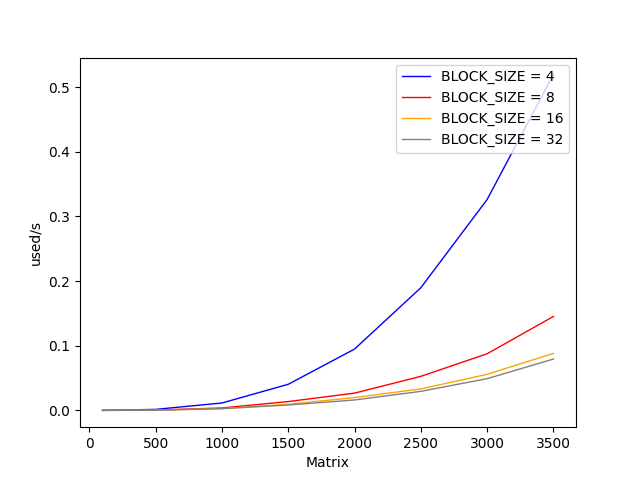
\includegraphics[scale=0.5]{3s}
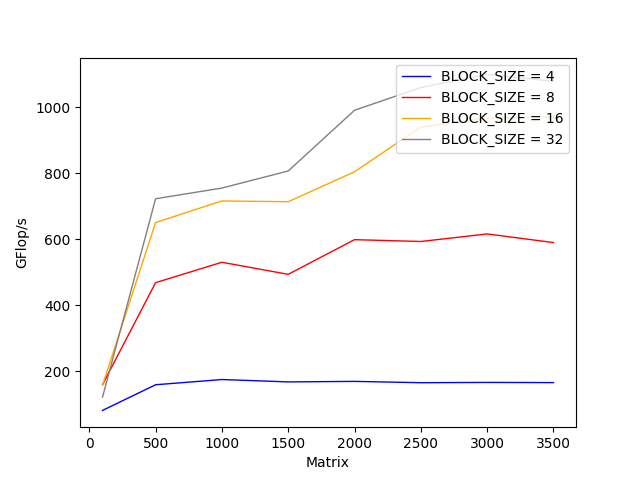
\includegraphics[scale=0.5]{3g}

The BLOCK\_SIZE for 32 is the faster. Although the increase is not obvious compared to 32, but as the width of Matrix increases, it will do more.
And I try the BLOCK\_SIZE for 64, but it doesn't work, so a block have up to 1024 (32*32) threads (or more) in the device RTX 2060 SUPER?


\begin{center}
    \Huge{That's all}\\
    \Huge{End!}\\
\end{center}

\end{document}
